\section{Implementation}
\def \kapitelautor {Christoph Führer}

\subsection{Structure of the System}
The whole structure of the system is held extremely simple. That was one of the major concerns we had while developing the software because the success of the application relies a lot on it being intuitive and simple. Therefore it is just a sole program in a single window which gives the user a very visceral feeling when using the application.

All actions done in the background, for example creating links, database management, assigning tags, \ldots{} are not visible for the user due to the fact that it would further increase the risk of him being overwhelmed by Octotagger's functions.

\subsection{The final product}
After a lot of hard work we managed to finish the first version of Octotagger but what were our thoughts behind it while developing? As mentioned above one of the major tasks we set ourselves was to make it as intuitive as possible. That surely sounds nice but what does it actually mean?

In our case it means that the user has to understand the basic structure of the application quickly, without being overwhelmed by its features. He should be able to easily understand the main points of our software so he can start using it right away. That means that any difficulties that the user could experience will hinder his enjoyment and therefore results in a loss of intuitiveness. The absolute key point on this topic was that the application has to be easy to use for the user, not the other way around.

The accomplish that we had the idea to make the whole program as native as possible. We want to give the user the impression that he is using an application which feels like it is coming directly from the operating system. As if it is already embedded from the start. The user should get the experience that there is not even a third party involved. He should get the feeling that our application is just an extension to his basic file manager, an enhancement which is easy to use and simplifies his file management.

Furthermore, we tried to make every single action that the user may take extremely simple. Basic commands that the user is used to from other popular programs and operating systems work exactly the same in Octotagger. You want to rename a file? Just press \textit{F2}. Refresh the View? Press \textit{F5}. All these classic commands that many of the users are already using by default are implemented precisely in our application so there won't be any complications when using Octotagger. For all the people who are not used to any shortcuts, there are also buttons for every action and context menus implemented.

\subsubsection{Initial startup}
When you run Octotagger for the first time this is what you will see:

\begin{center}
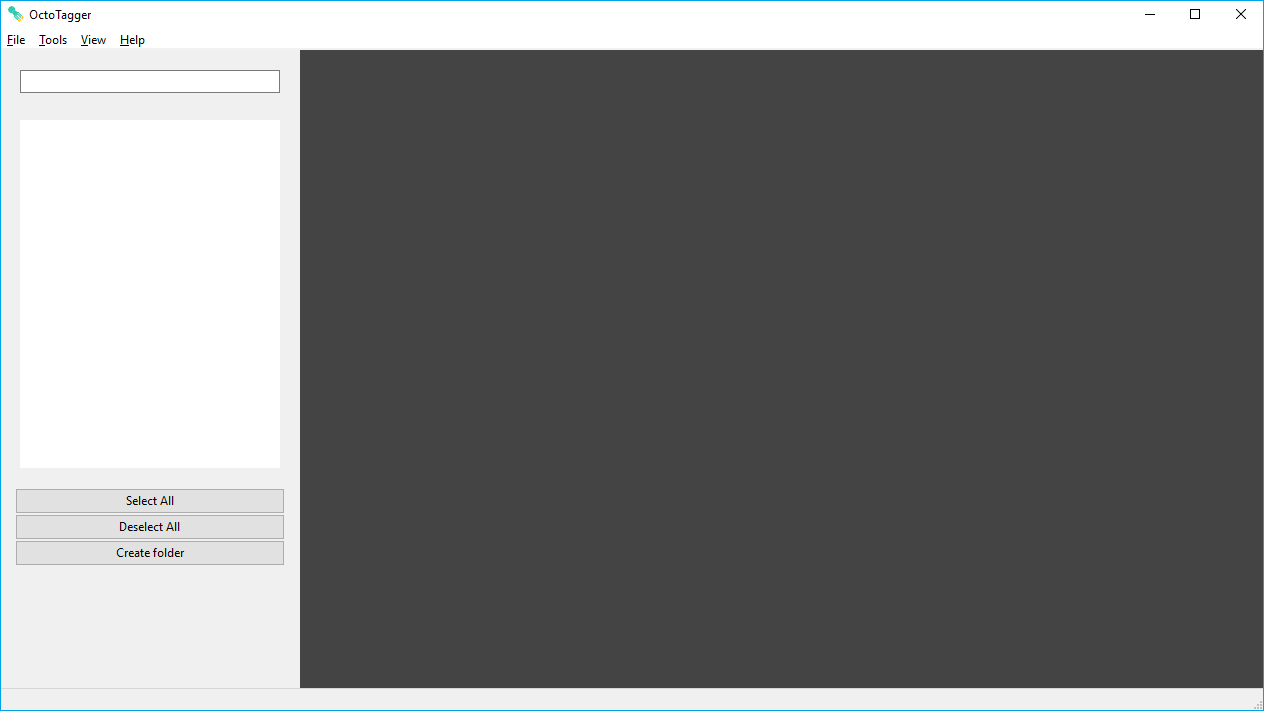
\includegraphics[width=\linewidth]{pp_04}
\small{Startup look of the user interface}
\end{center}


Looks pretty blank doesn't it? That is because there are neither files imported nor tags assigned yet. To do so, you have to click on the \textit{File}-Tab and then on one of the file import options.

The next step is to assign tags to the imported files. This is done by selecting the files you want to be tagged, clicking on the tag-bar in the top left corner, typing in a tag and finally pressing enter. Your files are now tagged, which can be seen in the tag-pane right below the tag-bar.
This is an example look of how your application may look after you are done with the tagging process.

\begin{center}
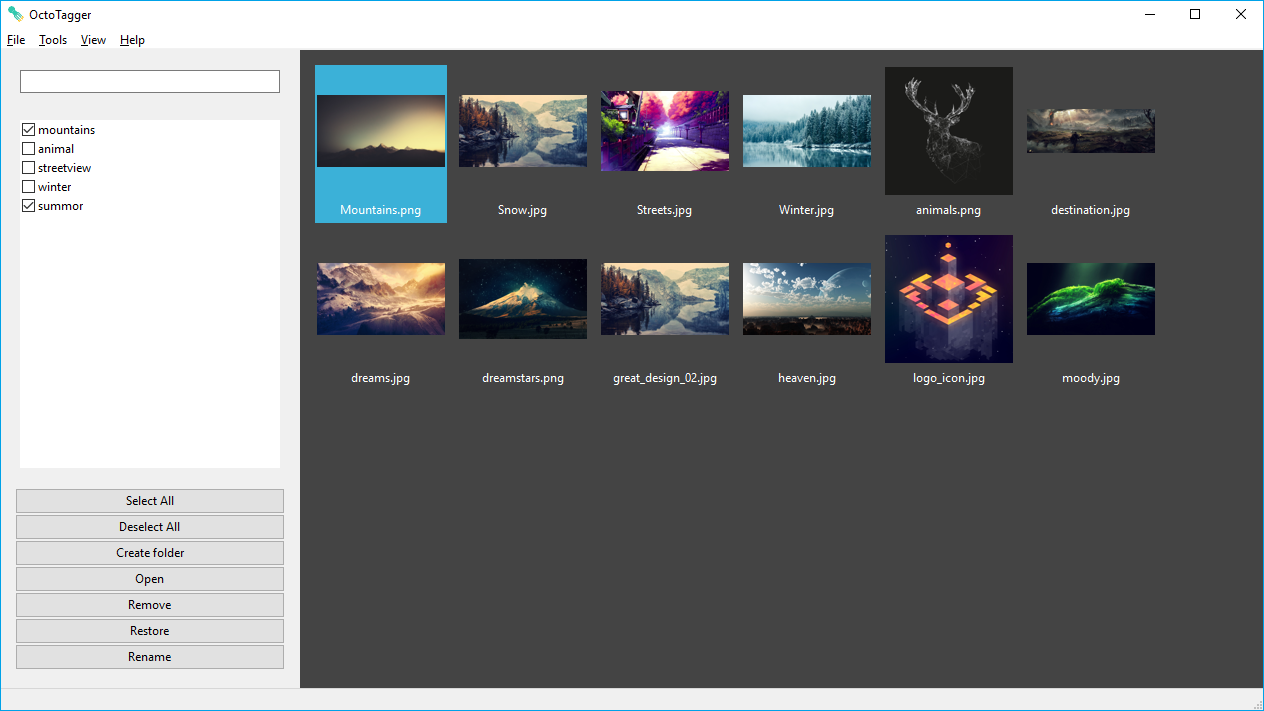
\includegraphics[width=\linewidth]{pp_03}
\small{User interface after importing and tagging}
\end{center}


Great! From this point onwards you are to use Octotagger to the fullest. You can now utilize and enjoy all the different functions that are explained in the execution chapter.

\subsubsection{Behind the scenes}
Now that you have seen how the program looks on the outside, let's take a look at the backend. This is what your folder structure will look like right after downloading Octotagger:

\begin{center}
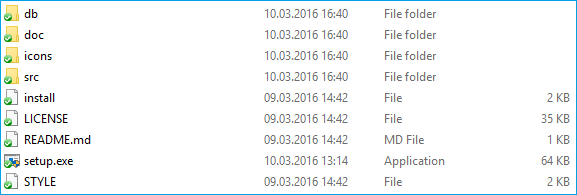
\includegraphics[width=\linewidth]{pp_06}
\small{File structure of Octotagger before installing}
\end{center}


It really is as simple as it looks. The \textit{db}-folder contains database and SQL files, in the \textit{doc}-folder is our documentation and user manual, our Python files are in the \textit{src}-folder and the \textit{icons}-folder contains logos and other images that are displayed in the application.

\subsection{Installation}
Installing Octotagger is easy. It has to be. 

\paragraph{}
The software is not installed yet though. The first step after downloading the software from our Website \href{"http://www.octotagger.co/"}{www.octotagger.co} would be to run the \textit{setup.exe}. Luckily, this was already the only step that needs to be done! Afterwards your directory will look like this:

\begin{center}
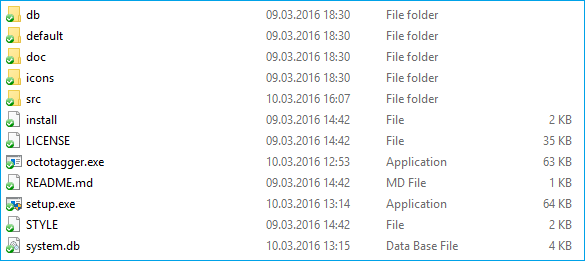
\includegraphics[width=\linewidth]{pp_05}
\small{File structure of Octotagger after installing}
\end{center}


The following things have changed:
\begin{itemize}
	\item A new folder named \textit{default} has been created. It embodies your default gallery which contains a Data Base File, a \textit{files}-folder, where your imported files are saved in and a \textit{thumbnails}-folder in which the thumbnails for you imported files are saved.
	\item Another Data Base File has been created
	\item The Octotagger.exe has been created
	\item A shortcut on the desktop has been created
	\item You are now able to run Octotagger!
\end{itemize}

However, it is worth mentioning that you have to execute the setup file with administrator rights on Windows because of the simultaneously created Windows Symlink service which is also explained more in depth in the Execution chapter. The reason for this is that on Windows it is needed to build a service which handles the link creation, due to the fact that Windows does not allow this feature without special permission. By creating a Windows service you only have to grant these rights once and are fine for as long as you keep it installed. If you want to gain a deeper understanding about this topic please consider looking at the \textit{Pywinlink} Module chapter in the execution part.

\subsection{Goals}
We are proud to tell that all Must-Goals have been achieved! The Software is running smoothly and we are all utterly satisfied with the outcome of a year of developing Octotagger. Of course there have been some complications, challenges and other things that did not go exactly according to plan but all in all we did not have any major troubles and a pleasant time engineering the software.

If you wish to receive more information about which goals, including the optional ones, have been achieved and which ones did not we recommend reading the analysis in the \textit{Evaluation} chapter. There you will also find information on how we planned the whole project in contrast to how we eventually carried it out.






















